% CSE 521S Final Report
% A Parking Guidance and Information System for TinyOS
% By Matthew Lindsay, Patrick McBryde, Michael Schultz

\documentclass{acm_proc}
\usepackage{hyperref}
\usepackage{url}
\usepackage{graphicx}

\begin{document}

\title{A Parking Guidance and Information System for TinyOS}
\subtitle{CSE 521S Final Report}

\numberofauthors{3}
\author{
\alignauthor Matthew Lindsay\\
% 2nd. author
\alignauthor Patrick McBryde\\
% 3rd. author
\alignauthor Michael Schultz\\
\and
\affaddr{Washington University in Saint Louis}\\
}

\maketitle

\begin{abstract}
The Internet is able to provide up to the minute updates on traffic
conditions and provide motorists with detailed mapping and directions for
nearly any destination.
However, once a driver arrives at their destination, they must still
search for a parking space.
This wastes fuel and time, as well as causing traffic buildup and
contributing to the urban heat island effect.
We believe that Wireless Sensor Networks (WSN) can be used to aide in these
problems.
Drivers would be able to access up to the minute information about parking
from their home computer or smart phone.
Our system can provide high frequency updates for, we believe, a cost lower
than current implementations.
Most commonly, expensive induction loops or other, more permanent systems
must be installed, and only provide entrance and exit information for
parking structure.

Modern ``Intelligent Transportation Systems'' (ITS) are a mix of systems
that gather various data metrics from transportation areas (parking lots,
streets, alleyways, etc.), aggregate this data together, and present
coherent information to the end-users of the system.
Orchestrating such a system presents several challenges at each level.
How do you gather the data and at what granularity?
Where does the data go once gathered and can it be useful to anyone?
If it can be useful, how can it be presented to end-users to provide
accurate and simple-to-interpret content?
This paper presents and explains our decisions in developing a ``Parking
Guidance and Information'' (PGI) system for TinyOS.
\end{abstract}

\section{Introduction}
When Tim Berners-Lee introduced the World Wide Web to the world in 1991, he
commented that,
\begin{quote}
``[The World Wide Web] could start a revolution in information
access.''
\end{quote}
In the past 20 years there has been a huge wealth of information placed
online for anyone to access anywhere.
The revolution is just beginning however, there is still an incredible
amount of ``now'' information that simply isn't available online yet.
We want to use wireless sensor networks in order to push more ``now''
information online, in this project we target parking lot data to simplify
a driver's life when traveling.

Driving to new destinations always brings some level of stress and
uncertainty.
Questions like: where am I going, what do the roads and intersections look
like, what side of the road is the place on, and where do I park are common
when traveling to new locations.
Luckily, mapping technology brings us the answers or at least partial
answers to some of these questions.
In the past decade there has been huge growth of web-based mapping
technology, allowing these questions to be answered even more fully.
For example, Google Maps allows you to get directions from point A to point
B, and in the past 5 years has introduced Street
View~\cite{vincent:streetview} to their interface.
Street View allows a user to view the roads they will be traveling on from
an in-car perspective.
This removes much of the uncertainty when driving, leading to less
confusion, a better experience, and potentially fewer accidents.

However, there is still more that can be done.
Once you've arrived at your destination you must find where to park.
This can be a hassle for those unfamiliar with an area or
during peak hours when there may not be a parking space nearby.
Parking Guidance and Information Systems (PGIS) allow drivers to quickly
evaluate where empty parking spaces may exist~\cite{sakai:pgi-toyota}.
Traditional PGI Systems just count the number of cars that enter and exit a
designated area, displaying the number of spots available in that area to a
driver.
These systems are imprecise, costly, and are difficult to integrate with
other technologies.

This paper presents our experiences building a PGI System on the
TelosB/TinyOS platform.
By using motes, it is possible to deploy a single sensor for each parking
space allowing more detailed information about an entire parking lot.
Moreover, with proper sheltering, these sensors can be mounted on the
surface of a parking lot instead of cutting into the lot and installing an
inductive loop to detect vehicle presence.
We can also take advantage of the wireless multi-hop routing abilities of
TinyOS-based motes to avoid costly wiring and enable a heterogeneous mix of
sensors.
Combining these aspects gives a system is able to be more precise, lower
cost, and easily integrated with future technologies.

The remainder of this paper is as follows.
Section~\ref{sec:goals} defines the goals of this project more fully.
Section~\ref{sec:design} presents and explains the high-level architecture
of our PGI System and details the hardware and software used during the
course of this project.
Section~\ref{sec:experiment} talks about how we convinced ourselves that
the system worked correctly and, if we have more resources, could scale up
as needed.
Sections~\ref{sec:related} and~\ref{sec:lessons} give an overview of
related works and lessons we learned during this project.
Finally, Section~\ref{sec:conclusions} concludes this paper with a
discussion of potential future work for this project.

\section{Goals}\label{sec:goals}

Since we believe other solutions to PGI Systems do not represent what
modern technology is capable of, our goals for this project are to build a
PGI System that can be easily deployed at a low-cost while aggregating the
data to a single location and integrating it with user-facing technology to
provide a rich user experience.
In short, we plan to answer the following questions:
\begin{itemize}
	\item How do you gather parking data and at what granularity?
	\item Where does the data go once gathered and can it be useful to
	anyone?
	\item How can it be presented to end-users to provide accurate and
	simple-to-interpret content?
\end{itemize}

Our goals for the hardware involve prototyping a low-cost, wireless system
that functions with a heterogeneous sensor suite.
This can be accomplished by using sensors with standard connection ports,
allowing the system to be customized with different sensing methods.
We can also take advantage of the built-in sensors to provide drivers
with advanced feedback, such as headlight detection.
Lastly, our project should be available for current parking structures to
use.
Therefore, it must make use of the wireless capabilities of the mote
platform, reducing installation costs by removing the need for costly
wiring.

Once our system is installed, we can collect the data at a base station,
located at the parking structure, which will interact with both the WSN and
the Internet.
Communication between the base station and the network will rely upon
Collection Tree Protocol (CTP), a robust method of point-to-sink wireless
communication.
Our base station then communicates with a computer via USB and sends
the data to the Internet.

\section{Design}\label{sec:design}

\begin{figure}
    \begin{center}
		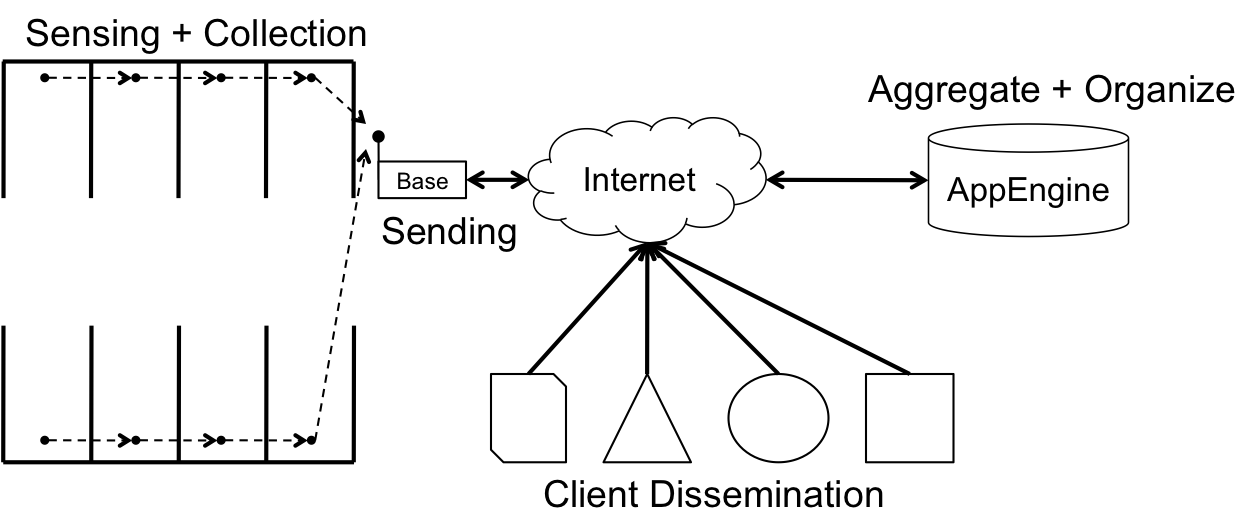
\includegraphics[width=\columnwidth]{figures/high-level}
	\end{center}
	\caption{High-level view of our PGI System. A base station at the lot
	sends data over the Internet to our aggregator, which end-users can
	query.}
	\label{fig:high-level}
\end{figure}

Figure~\ref{fig:high-level} shows a high-level view of the infrastructure
of our PGI System.
Our system begins with a parking lot with each space equipped by a sensor
built on the TelosB/TinyOS platform.
Data is collected at a base station and then sent over the Internet to our
backend.
When our backend receives the data it updates and logs the changes to the
data store and organizes the lot information.
Once the data is stored, clients can query the backend, getting up to the
minute information about a specific lot and lots in the vicinity.

To present the system, we first introduce our API that ties the two major
components (sensing and aggregation) together.
Once the API is in place, we explain the hardware sensing design and then
the aggregation and dissemination system.

\subsection{A RESTful API}

REpresentational State Transfer (REST) is an abstract model for building
large-scale web services~\cite{pautasso:restful}.
The principles of a RESTful architecture are an identification of resources
through a URI, a ``pure'' HTTP interface, and self-contained hyperlinks.
This section describes how we achieved these principles.

Our URI scheme is straight-forward.
Each lot is given a unique identification consisting of alphanumerics and
the underscore (\_) character.
When attempting to access a specific lot, that identifier is part of the
URI (i.e.,
\texttt{http://<host>/lot/wustl\_millbrook/}
identifies the Milbrook lot on Washington University's campus).

\begin{figure}
    \begin{verbatim}
[
  {
    "space_id": 8,
    "is_empty": false,
    "magnet": 218,
    "sonar": 114
  },
  ...
]
\end{verbatim}
	\caption{Client to server JSON data.}
	\label{fig:clientserverjson}
\end{figure}

Requests concerning this lot must go through its respective URI.
Requests use one of the HTTP verbs of \texttt{GET}, \texttt{PUT}, or
\texttt{POST}.
A \texttt{GET} request simply returns the information for the requested URI
in either the HTML or JSON~\cite{crockford:json} format.
A \texttt{PUT} request attempts to store updated status information to the
lot.
This request contains the list of parking spaces to update, their
identification and status, as well as any associated meta-information that
should be put in the datastore, an example of this can be seen in
Figure~\ref{fig:clientserverjson}.
Finally, a \texttt{POST} request handles the creation of new parking lots.

\begin{figure}
    \begin{verbatim}
{
  "lot_id": "wustl_snowway",
  "geo_pt": "38.650233,-90.313529",
  "timestamp": 1291946695.0
  "spaces":
  [
    {
      "space_id": "4",
      "is_empty": false,
      "timestamp": 1291946695.0,
      "extra_info": "sonar:55;magnet:201;"
    },
    ...
  ]
}
\end{verbatim}
	\caption{Server to client JSON data.}
	\label{fig:serverclientjson}
\end{figure}

As mentioned, a \texttt{GET} request on the parking lot identifier results
in either a HTML or JSON response.
An example of the JSON response can be seen in
Figure~\ref{fig:serverclientjson}.
The JSON response provides enough information for a client application to
identify the name of the lot, its location, the time of the most recent
activity, and the list of spaces.
Each space has a unique identifier, the status of that spot (full or
empty), the time it was last updated, and any additional information about
that spot (likely to be sensor readings at the last report).
A client can potentially combine this information with a virtual
representation of the lot's topography, then keep that representation
updated by periodically querying the server for new information.

With the API in place, we are able to tie an arbitrary sensor network into
our service (if it follows our description) and can provide rich
applications access to our information with ease and the possibility of
expansion.
We are now free to discuss the specifics of our hardware sensing platform
and our web application that presents the data.

\subsection{Hardware}

When choosing the hardware for our PGI system we had specific goals in mind.
The system must be low-cost, reliable, power efficient, and easily
customized to meet the needs of the specific structure or parking lot.
A primary focus of this system is to upgrade existing parking structures, not just add it to new construction.
Therefore our system must be capable of customizing sensors for different
environments.

For example, an induction loop sensor is typically the best sensor for
detecting the presence of a vehicle, but in a pre-existing structure you
must cut into the floor of every parking space to add them, a costly
procedure.
When adding an inductive loop system, the installation cost is more prohibitive
than that of the PGI system.
This customization is likely the most important requirement for the successful
adoption of our system by the parking industry.
By using wireless technology and supporting many different sensor types and
configurations we believe we can successfully implement this system in both
pre-existing and new parking structures.

\subsubsection{Parking Space Monitors}

The Parking Space Monitors (PSMs) need to be able to do more than just determine
if a vehicle is present in a parking space.
They must be able to run on a set of batteries for an extended period of
time, support multiple sensor types and interfaces, and wirelessly transmit
the required data to a base station for further processing.
For all these reasons we chose the Telos Revision B (TelosB) wireless
sensor module as the base for our PSMs.

\begin{figure}
    \begin{center}
		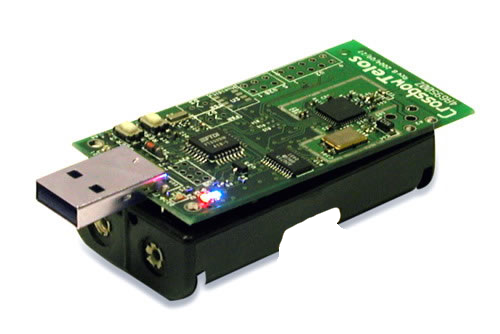
\includegraphics[width=\columnwidth]{figures/telosb}
	\end{center}
	\caption{Telos Revision B.}
	\label{fig:telosb}
\end{figure}

Shown in Figure~\ref{fig:telosb}, the TelosB provides many
features and sensors while still managing to use little power and support
fast wireless communications.  We chose the TelosB because it includes a
250 kbps IEEE 802.15.4 wireless transceiver; on-board temperature and light
sensors; low power consumption; an on-board antenna; simple
programming/collection interface; and a 10+6-pin expansion slot allowing
analog, digital, or serial connections~\cite{moteiv:telosb}.

The TelosB includes many different interfaces we could use to attach
sensors too.
These include analog to digital, UART, I2C, and digital connections, this
selection gives us a very flexible platform.
It's this flexibility that will make our system a viable option for parking
structures.

\begin{figure}
    \begin{center}
		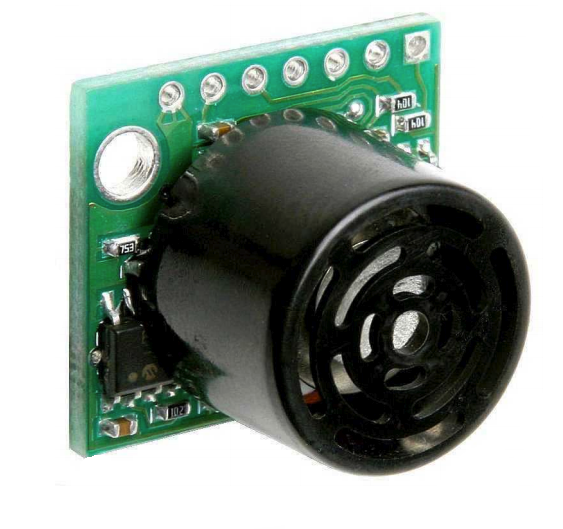
\includegraphics[height=1.5in]{figures/range_finder}
	\end{center}
	\caption{LV-MaxSonar\textsuperscript{\textregistered}-EZ1\textsuperscript{\texttrademark}
	by MaxBotix\textsuperscript{\textregistered} (hereafter ``EZ1'').}
	\label{fig:range_finder}
\end{figure}

There are many different types of sensors that could have been used to
monitor if a parking space is occupied or vacant.  These include infrared
range finders, pressure sensors, and inductive sensors.
We chose to use the
LV-MaxSonar\textsuperscript{\textregistered}-EZ1\textsuperscript{\texttrademark}
by MaxBotix\textsuperscript{\textregistered} (hereafter ``EZ1'')
because of its price and feature set.
The EZ1 supports a wide range of standard supply voltage inputs.
This allows us a great deal of flexibility in choosing how to power the
EZ1.
It can detect objects from 6 inches to 254 inches.
This is enough range to cover the complete parking space.
The EZ1 supports many output formats including pulse width, analog voltage,
and serial digital.
This gives us multiple ways to connect the same sensor depending on the
environment~\cite{maxbotix:maxsonar-datasheet}.

\subsubsection{Base Station}
A MacBook Pro was used as the base-station in this project.
However, keeping with our theme of low-cost, we kept the
requirements of the base station to a minimum by only using features found
in any low-end Unix or Linux computer.
The only requirements of the base station are that it be capable of
connecting to the Internet and that it provides a USB connection.
Because video is not a requirement, we would recommend a small, power
efficient and cost effective plug
computer~\footnote{\url{http://www.wikipedia.org/wiki/Plug_computer}}.

The base station must be able to have IEEE 802.15.4 communications with the
PSMs, this can be achieved by connecting a TeloB via USB and using a simple
serial connection to allow the two devices to communicate.  

\subsection{Collection Software}

\subsubsection{Parking Space Monitors}

The PSMs are powered by TinyOS.
We chose TinyOS because it fully supports the TelosB and provides many
features that rapidly speed-up development.
These include mesh networking and communication protocols as well as native
support built in for all the connection interfaces described earlier.

The PSMs receive configuration data from the base-station and then begin
monitoring sensor values.
Every sample period the PSMs sample the sensors ten times and average the
values.
Those values are then wirelessly transmitted to the base-station every
fifteen seconds.
One of our key design goals was wireless reliability.
Packets containing sensor details must always make it back to the base station for processing.
This can be very difficult in dynamic environment such as a parking
structure, especially a multi-floored garage where line of site is
impossible, and transmissions will attenuate through the industrial walls present in the structure.
Therefore, alternative methods of packet forwarding must be introduced in
order for the system to be able to operate with a single, centrally located
base station.
In this project, we attempted to use Collection Tree Protocol (CTP).

CTP is a dynamic point-to-sink routing protocol, which creates a tree
topology for the network through which all packets travel to the base
station, known as the root node or sink.  By creating this tree based
topology, motes dynamically create an efficient routing method for
collecting all data at a centralized point.  CTP does not handle
point-to-point communication, though it does provide support for
broadcasting to all nodes~\cite{tep123:collection-tree-protocol}.
In our final implementation, due to a miscommunication about integrating
the various parts of the project, CTP was left out.
However, initial tests of a non-trivial CTP network gave indications that
it would function well within our project.

\subsubsection{Base Station}

The base station software has multiple functions.  It was written in C so
as to be compatible with most current versions of Unix or Linux.
It is responsible for configuring the PSMs, monitoring their status, collecting data from them, and sending the collected data to the aggregation software over the Internet.

Since the base station needs to communicate with the motes over IEEE
802.15.4, a TelosB is connected via USB as part of the base station.
The TelosB is running the default BaseStation app (included with the TinyOS
install) with only minor tweaks to support CTP.

The base-station has the ability to send configuration packets to the PSMs.
It is through this configuration process that the PSMs are assigned their
parking space IDs.
The configuration packet structure was designed to be easily extended to
support future needs.
For example, the base station could adjust sensor read rates or data
transmission rates based on the time of day to increase PSM battery life.

The base station's primary purpose is to collect sensor readings from the
PSMs and relay it to the aggregation software.
The data is encoded as a JSON packet (as seen in
Figure~\ref{fig:clientserverjson}) and transfered via HTTP \texttt{PUT} to
the backend for processing.

\subsection{Aggregation Software}

Data leaving the base station of a parking lot is directed over then
Internet to our aggregation software hosted on Google's
AppEngine~\cite{google:appengine}.
We decided that AppEngine was an appropriate choice for several reasons:
\begin{itemize}
	\item The service is free for light usage (testing and development).
	\item It provides a Python programming environment.
	\item It scales up easily with large datasets.
\end{itemize}

We need easy scalability if we are to have one sensor per parking space for
every parking lot.
Thus our backend must be able to accept, store, and recall large amounts of
current and historical data.
A traditional server model may have worked for this prototype, but if the
project starts scaling up we would quickly start running into barriers.
AppEngine scales with demand due to their use of a data store built on top
of Bigtable~\cite{google:bigtable}.
Though transparent to users of our system, this non-SQL based data store
forces some differences from a SQL based data store.

While queries look like SQL, they are actually ``GQL,'' a SQL-like
language.
In general this does not bring any problems, but because of the
organization of the data store imprecise queries are not acceptable.
You must know the data you are looking for.
You cannot SELECT one or two columns from a row, you
must take the entire row or an identifier for the row.
As such, proximity searches are difficult because there is not concept of
``similar'' or ``like'' queries.
You either know how to find the data or you can't find the data at all.
However, with the help of the Geomodel API~\cite{geomodel} we can
use geohashing for proximity searches.
This allows the end-user to identify nearby parking areas.

\subsubsection{Frontend}

Our prototype frontend is an HTML interface that allows viewing information
about a parking lot.
The user can select a lot and our frontend provides a map of the area and
marks lots within a two mile radius.
It also displays a ``health'' indicator giving an approximate empty-to-full
ratio, as well as a percentage and a list of full spaces and their usage
duration.

\begin{figure}
    \begin{center}
		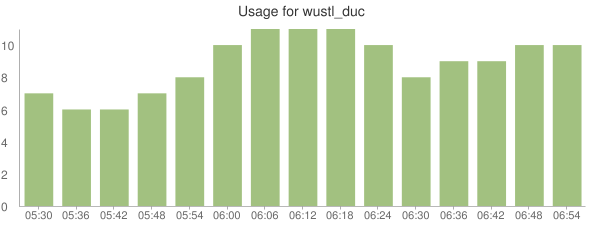
\includegraphics[width=\columnwidth]{figures/fullness-chart}
	\end{center}
	\caption{Example of a usage chart for the 5:30am--7:00am time slot.}
	\label{fig:fullness-chart}
\end{figure}

We also provide a chart to indicate the average fullness of a lot over a
time frame.
For example, Figure~\ref{fig:fullness-chart} shows the average fullness of
the ``DUC'' lot from 5:30am until 7:00am.
At the 6:06am time slot there are 11 spaces being used, however only 20
minutes earlier only 6 spaces are being used.
This information allows a commuter, or one time visitor, to find that by
arriving a little earlier they have a much greater chance of easily finding
a parking space.

\section{Experiment}\label{sec:experiment}

Since our system was split into two major components, we were able to test
both somewhat independently. 
The first component included physically sensing the vehicle and relaying
the data to the backend~\footnote{A video is available at
\url{http://www.youtube.com/watch?v=cE2xn1PHDlI}.}.
The second component involved testing the backend works for extended
periods of time and correctly logs/recalls historical data.

\subsection{Sensing and Sending}

\begin{figure}
    \begin{center}
		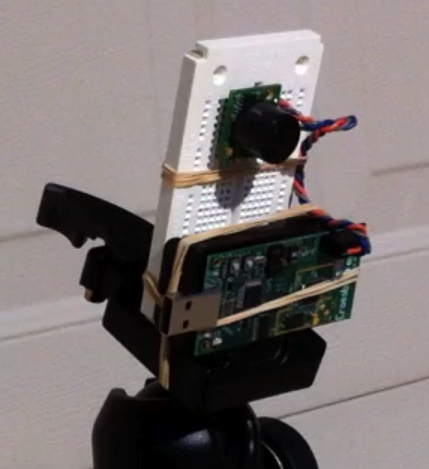
\includegraphics[width=\columnwidth]{figures/parking_sensor}
	\end{center}
	\caption{Parking Space Monitor on tripod for testing.}
	\label{fig:parking_sensor}
\end{figure}

A large amount of testing was performed on the sensing and sending portion
of this project.
Figure~\ref{fig:parking_sensor} shows a PSM mounted on a
tripod.
This set-up was used to test the system with an actual vehicle.
This testing found issues with the sensing range of our PSMs.
The EZ1 should support a distance up to 254-inches, however we
were only able to detect a vehicle up to approximately 120-inches (10
feet).
Though this did not cause an issue detecting a vehicle, it could be an
issue with detecting smaller objects such as motorcycles.
More testing and analysis would need to be performed to determine if the
ten foot range of the EZ1 would really be an issue.
It was determined while testing this issue that it was caused by the supply
voltage to the EZ1.
The EZ1 will support a supply voltage of 2.5V - 5.5V.
We chose to power the EZ1 using the TelosB analog supply which
supplies about 3.1V.
When we used an external supply to test just the EZ1 at 5V it had a much
greater range compared to 3.1V.
If after more testing it is determined to be an issue, there are solutions
such as using an external power supply for the EZ1 or possibly mounting the
sensor above the space to cover a greater area of the space. 

\subsection{Backend and Frontend}

Since it was not feasible to test a large scale deployment due to cost,
time, and logistical constraints a base station simulator was developed.
Instead of interacting with a sensor network for gathering data, the
simulator was designed to generate a number of changes to a lot every one
to two minutes.
The  changes include modifying the status of a random number of parking
spaces with some weight attached to the likelihood of a space becoming empty
for a time interval.
For example, during the overnight hours there only a 16\% chance of a
parking space becoming full causing the overnight hours to present less lot
usage.

This simulator helped test the ability of the backend to continue to be
stable over a number of hours while periodically inserting new log
information and maintaining the current status of a parking lot.
It also helped generate large amounts of data for testing the analytics
portion of our frontend (charting for time periods).

\section{Related Work}\label{sec:related}

There are other proposals and existing systems for parking guidance and
information, here we'll discuss and differentiate ourselves from these
systems.

Signal-Park, uses sonar sensors above each parking spot to detect the
presence of a vehicle~\cite{pgi:signal-park}.
Approximately three times per second, the sensor is queried to determine
vehicle presences and updates a central computer.
This system uses serial lines to connect each sensor with the central
computer, leading to more costly deploy.
It also appears to be limited to the parking lot that it is deployed in and
lacks the ability to aggregate the information for others to benefit.
It would certainly be possible to improve the connectivity of this system
to integrate with our backend aggregation system to take advantage of
existing installations.

Streetline, a startup in the San Francisco area, uses a wireless network to
link all the sensors together~\cite{pgi:streetline}.
The Streetline system has recently (Summer 2010) begun to roll out sensors
and upgraded meters for select areas in the San Francisco
area~\cite{wired:streetline, sfpark}.
This system uses surface (and sub-surface) sensor mounts that contain a
wireless transmitter and a magnetometer for vehicle detection.
Status information is sent to a central aggregation server where users can
see the status of street parking via their web browser, text message, or
smart phone; it also allows municipal workers to identify vehicles that
have not paid fully.
Presuming the Streetline trial is successful and the system expands, our
system and their system should be able to integrate with little effort and
could be seen as competitors.
We view this a positive, as it demonstrates that our project is a useful
idea with potential buyers available.

%There has also been a proposal to use existing security cameras with a view
%of a parking lot to detect vehicular presence~\cite{lin:vision-parking}.
%The results of their experiment, while decent for their scenario, seem
%unlikely to generalize to other systems.
%While it may be true that some lots have existing surveillance cameras, the
%paper also observes that cameras should be mounted higher for a more
%consistent and complete view of the lot.
%This goes against their principal of using existing cameras for the
%information, since additional cameras would have to be mounted to perform
%correctly (moving security cameras further from the observation area is
%probably not acceptable to the security officers).

\section{Lessons Learned}\label{sec:lessons}

If we were to pursue this project into the future we would probably modify
the design to allow a single TelosB to monitor multiple sensors.  The
ultrasonic range finder we used has multiple output types, one of them
being a two wire digital serial connection.
This allows for up to twelve EZ1s to be used with a single serial
connection.
This allows either two sensors per space to improve accuracy and monitor
six spaces per TelosB or continue with a single range finder per space and
monitor twelve parking spaces per TelosB.
This could greatly decrease the cost and power consumption of the overall
system.

Another interesting lesson was using Google's AppEngine for the backend.
The cost structure of AppEngine is set up to be free as long as resource
usage stays below a daily threshold.
After modifying the frontend to automatically update the lot usage, we
easily surpassed the daily threshold giving us two options: back the
AppEngine instance with some money to increase our limits or refactor the
code to be less resource intensive.
Luckily, we were able to find a few code optimizations that greatly reduced
the resources for the automatic update code putting us under the daily
allotment again.

\section{Conclusions and Future Work}\label{sec:conclusions}

This project created an extensible wireless sensor that is able to detect
the presence of a vehicle in a parking space.
That data is transferred from the sensor, to the base station, and over the
Internet to our backend aggregator.
Once at our backend, the data is logged and inserted into a scalable web
infrastructure.
At any point an end-user is able to query our web service to determine the
current fullness of a lot at their destination and, if desired, find the
fullness of lots that are near-by to their destination.
The end-user is also able to discover when the lot is likely to be most
empty or most full.
Moreover, through the use of a web-based API using the standard JSON
format, application developers can interact with our system hassle-free
allowing rich web apps, smart-phone apps, or data mining opportunities.

As with many projects, there are both many features that can still be added
and much research into the viability of deploying such a sensor network.
Feature-wise, the web API could support richer queries.
For example, the ability to select multiple date ranges for charting
allowing a user to view average aggregate data for the weekdays over the
past month to decide if a parking lot should expand.
Another option is to integrate our system with a mapping service and
combine up to the minute traffic reports to allow a user to plan their trip
while being mindful of the route, traffic conditions, and available
parking.
On the hardware side, a careful evaluation of battery life and how to
increase battery life would be helpful.
Stripping away unused components from the TelosB could help greatly as well
as integrating solar panels for power support and creating an external
casing to protect the sensitive electronics from the environment.

\bibliographystyle{abbrv}
\bibliography{report}

\end{document}
